\documentclass[letterpaper, 11pt]{article}
\usepackage{comment} % enables the use of multi-line comments (\ifx \fi) 
\usepackage{fullpage} % changes the margin
\usepackage{fancyhdr} % for footer
\usepackage[UKenglish]{isodate}% http://ctan.org/pkg/isodate for date format
\usepackage{wrapfig}
\usepackage[font={small,sf}]{caption}
\usepackage{float}%force tables/figs into certain placement
\usepackage{graphicx}%for figures
\usepackage[leftcaption]{sidecap}%for figure captions
\usepackage{subcaption}%for figures
\usepackage{hyperref}%for hyperlinks
\usepackage[font=small,labelfont=bf]{caption}%for captions
%\usepackage{natbib}	%for bibliography
\usepackage{placeins}%prevent images from floating into inappropriate sections
\usepackage{tabulary}%for table at the end, to get soft wrapping
%\usepackage[capbesideposition=inside,facing=yes,capbesidesep=quad]{floatrow}
\usepackage[]{textcomp}%for degree symbol
\usepackage{titlesec}%to change appendix headers
\usepackage[titletoc,toc,title]{appendix}%to change appendix headers
\usepackage{gensymb}%for degree symbol

\usepackage{epigrafica}%changes default font to epigrafica
\usepackage[LGR,OT1]{fontenc}

\def\labelitemi{--}

\pagestyle{fancy}
\renewcommand{\headrulewidth}{0pt}

\lhead{}
\chead{}
\rhead{}
\lfoot{Frost Entomological Museum}
\cfoot{}
\rfoot{SOP 01 - \thepage}
\renewcommand{\footrulewidth}{0.4pt}
\title{SOP 01: Collection Environment and Etiquette}
\author{Frost Entomological Museum Curator \& Interest Group}

\begin{document}
\cleanlookdateon %removed ordinal date
\maketitle
\thispagestyle{fancy}

\section*{Preamble}
This SOP describes the specimen storage environment and establishes rules that govern behavior in the collection room and interaction with specimens.

\section{Collection room rules}

These rules apply to 131 Headhouse III, the main collection room, but also other rooms where specimens are stored.
\begin{enumerate}
\item In order to discourage pests and eliminate the possibility of accidents, \textit{no food and drink are allowed}, not even water
\item In order to maintain the proper environmental conditions---cool ($\sim$70\degree{}F) and dry ($\sim$40\% RH)---and to keep specimens secure from pests and theft, \textit{all entry doors are to be kept closed at all times} 
\item In order to exclude pests, \textit{all cabinet doors and drawers must be kept closed} when not accessing the collection, and \textit{specimens must not be left out}
\item In order to keep the space clean and ready for any urgent task, all materials, supplies, and equipment must be put away at the end of each day
\item In order to maintain the integrity of the collection, \textit{do not remove specimens} without the Director or Collection Manager's permission
\end{enumerate}

\section{Collection storage environment}
\subsection{General organization and labeling}
Each section of the arthropod collection is organized alphabetically by taxon: Family, genus, species. The Collection Manager has templates for labels that are applied to cabinets, drawers, and unit trays. Unit tray header cards must be inserted into space between plastazote and tray wall; the card may be braced with insect pins. Unit tray header cards that list species names must also include author, year, and parentheses if appropriate.

\subsection{Dry specimens}
\subsubsection{Storage containers}
For pinned insects, the Frost Museum uses USNM-style cabinets (must seal tightly), drawers (must seal tightly), and unit trays (plastazote pinning medium, with sides taller than typical pin height). \\

\noindent{}Odonata are stored in paper triangles or with 3$\times$5 cards inside cellophane envelopes. These preparations are stored in archival cardboard boxes, arranged in herbarium-style cabinets.

\subsubsection{Curatorial considerations}
Pinned specimens should be organized efficiently in unit trays---tightly packed and in a straight line but not touching anything---ideally one species per tray. Labels should be oriented consistently, such that they can be read in one view (Figure \ref{labelorient}. One should be able to remove/insert a specimen into a tray without risk of touching other specimens or the tray itself.\\

\begin{figure}[ht!]
	\centering
  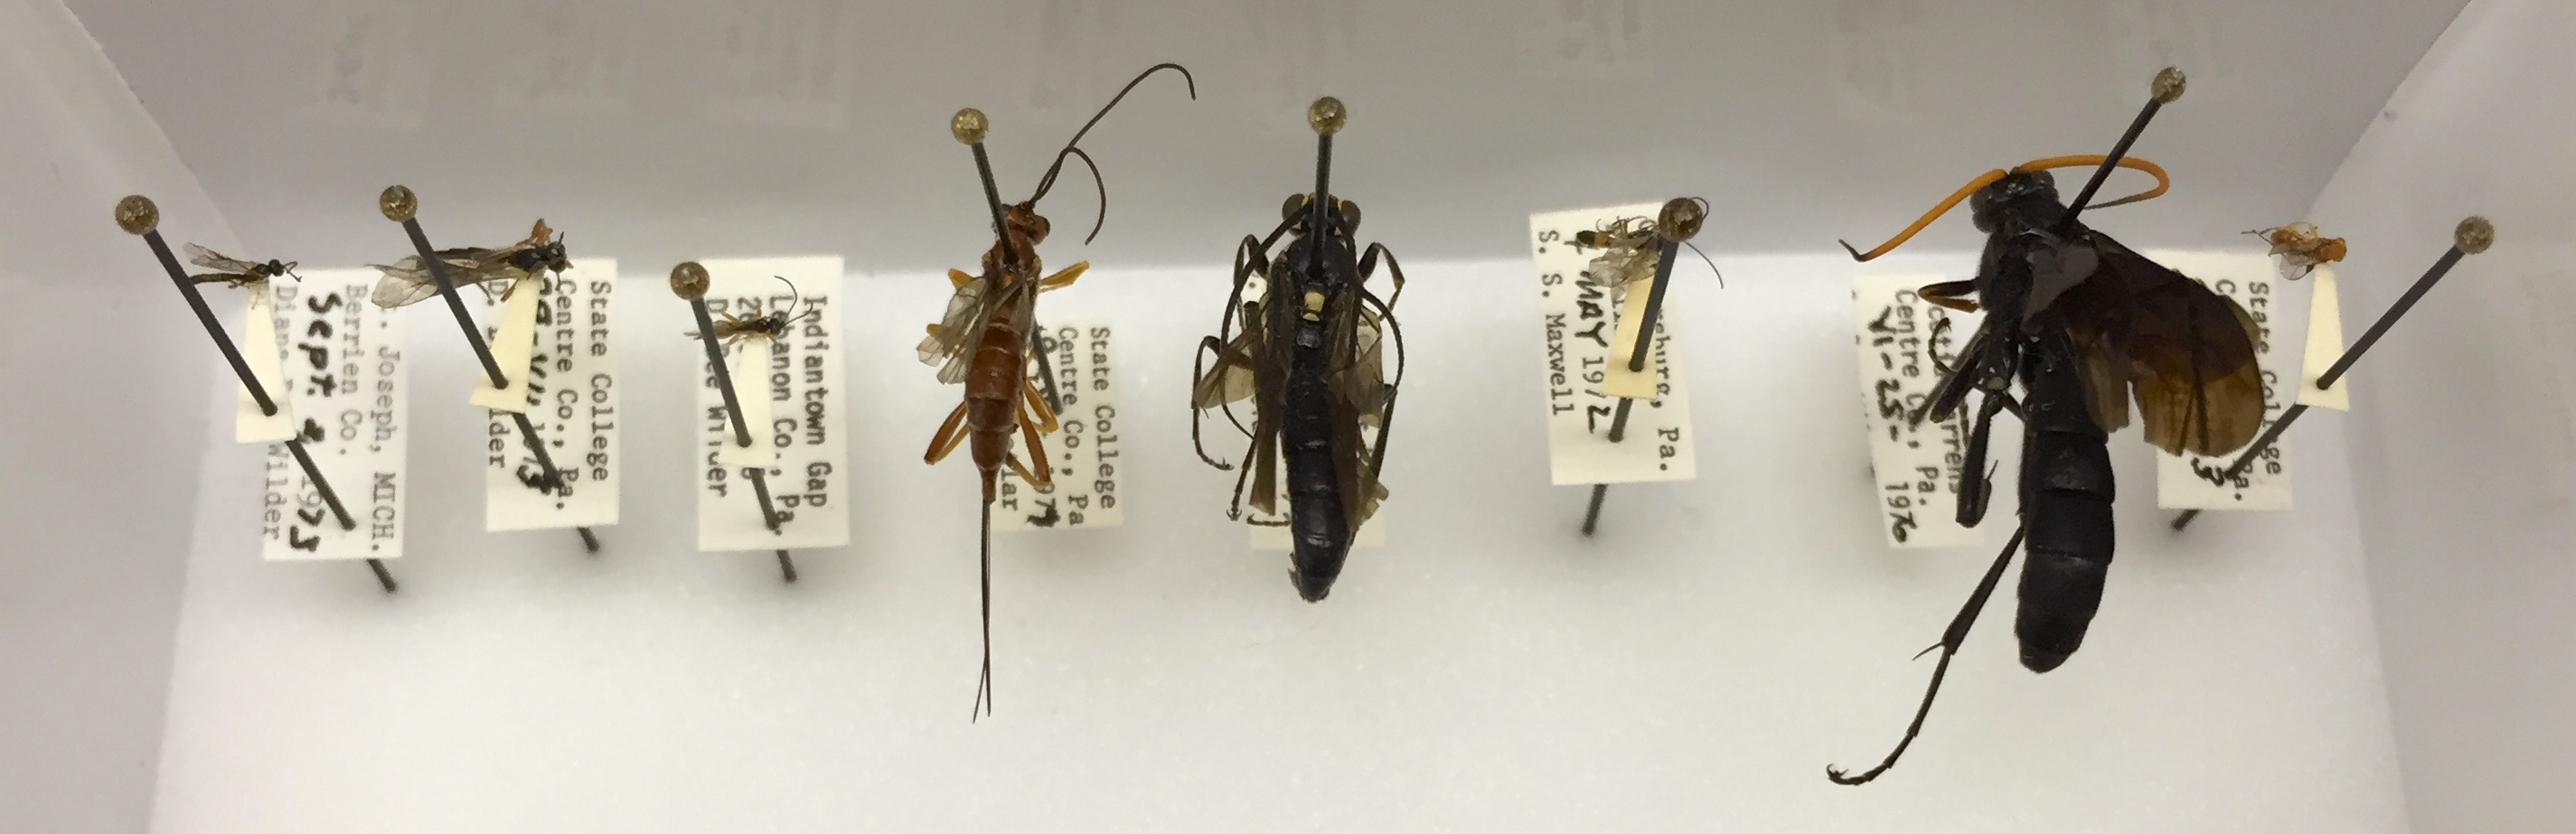
\includegraphics[width=0.75\textwidth]{labelOrientation}
  \caption{Heterogeneous specimen types organized inside a unit tray; note that labels are all oriented so that they can be read in one view. Specimens are placed in unit tray beginning in the upper left corner. Photo (CC BY 2.0) by Andy Deans.}
  \label{labelorient}
\end{figure}

\noindent{}Each drawer should have 25\% (ideally) free space, in the form of empty unit trays, to allow for growth and curation. Unit trays should fill each drawer, and any empty space between trays filled with archival plastazote spacers (Figure \ref{trayspacked}). Unit trays must not be allowed to slide around when a drawer is pulled or put back into a cabinet.\\

\begin{figure}[ht!]
	\centering
  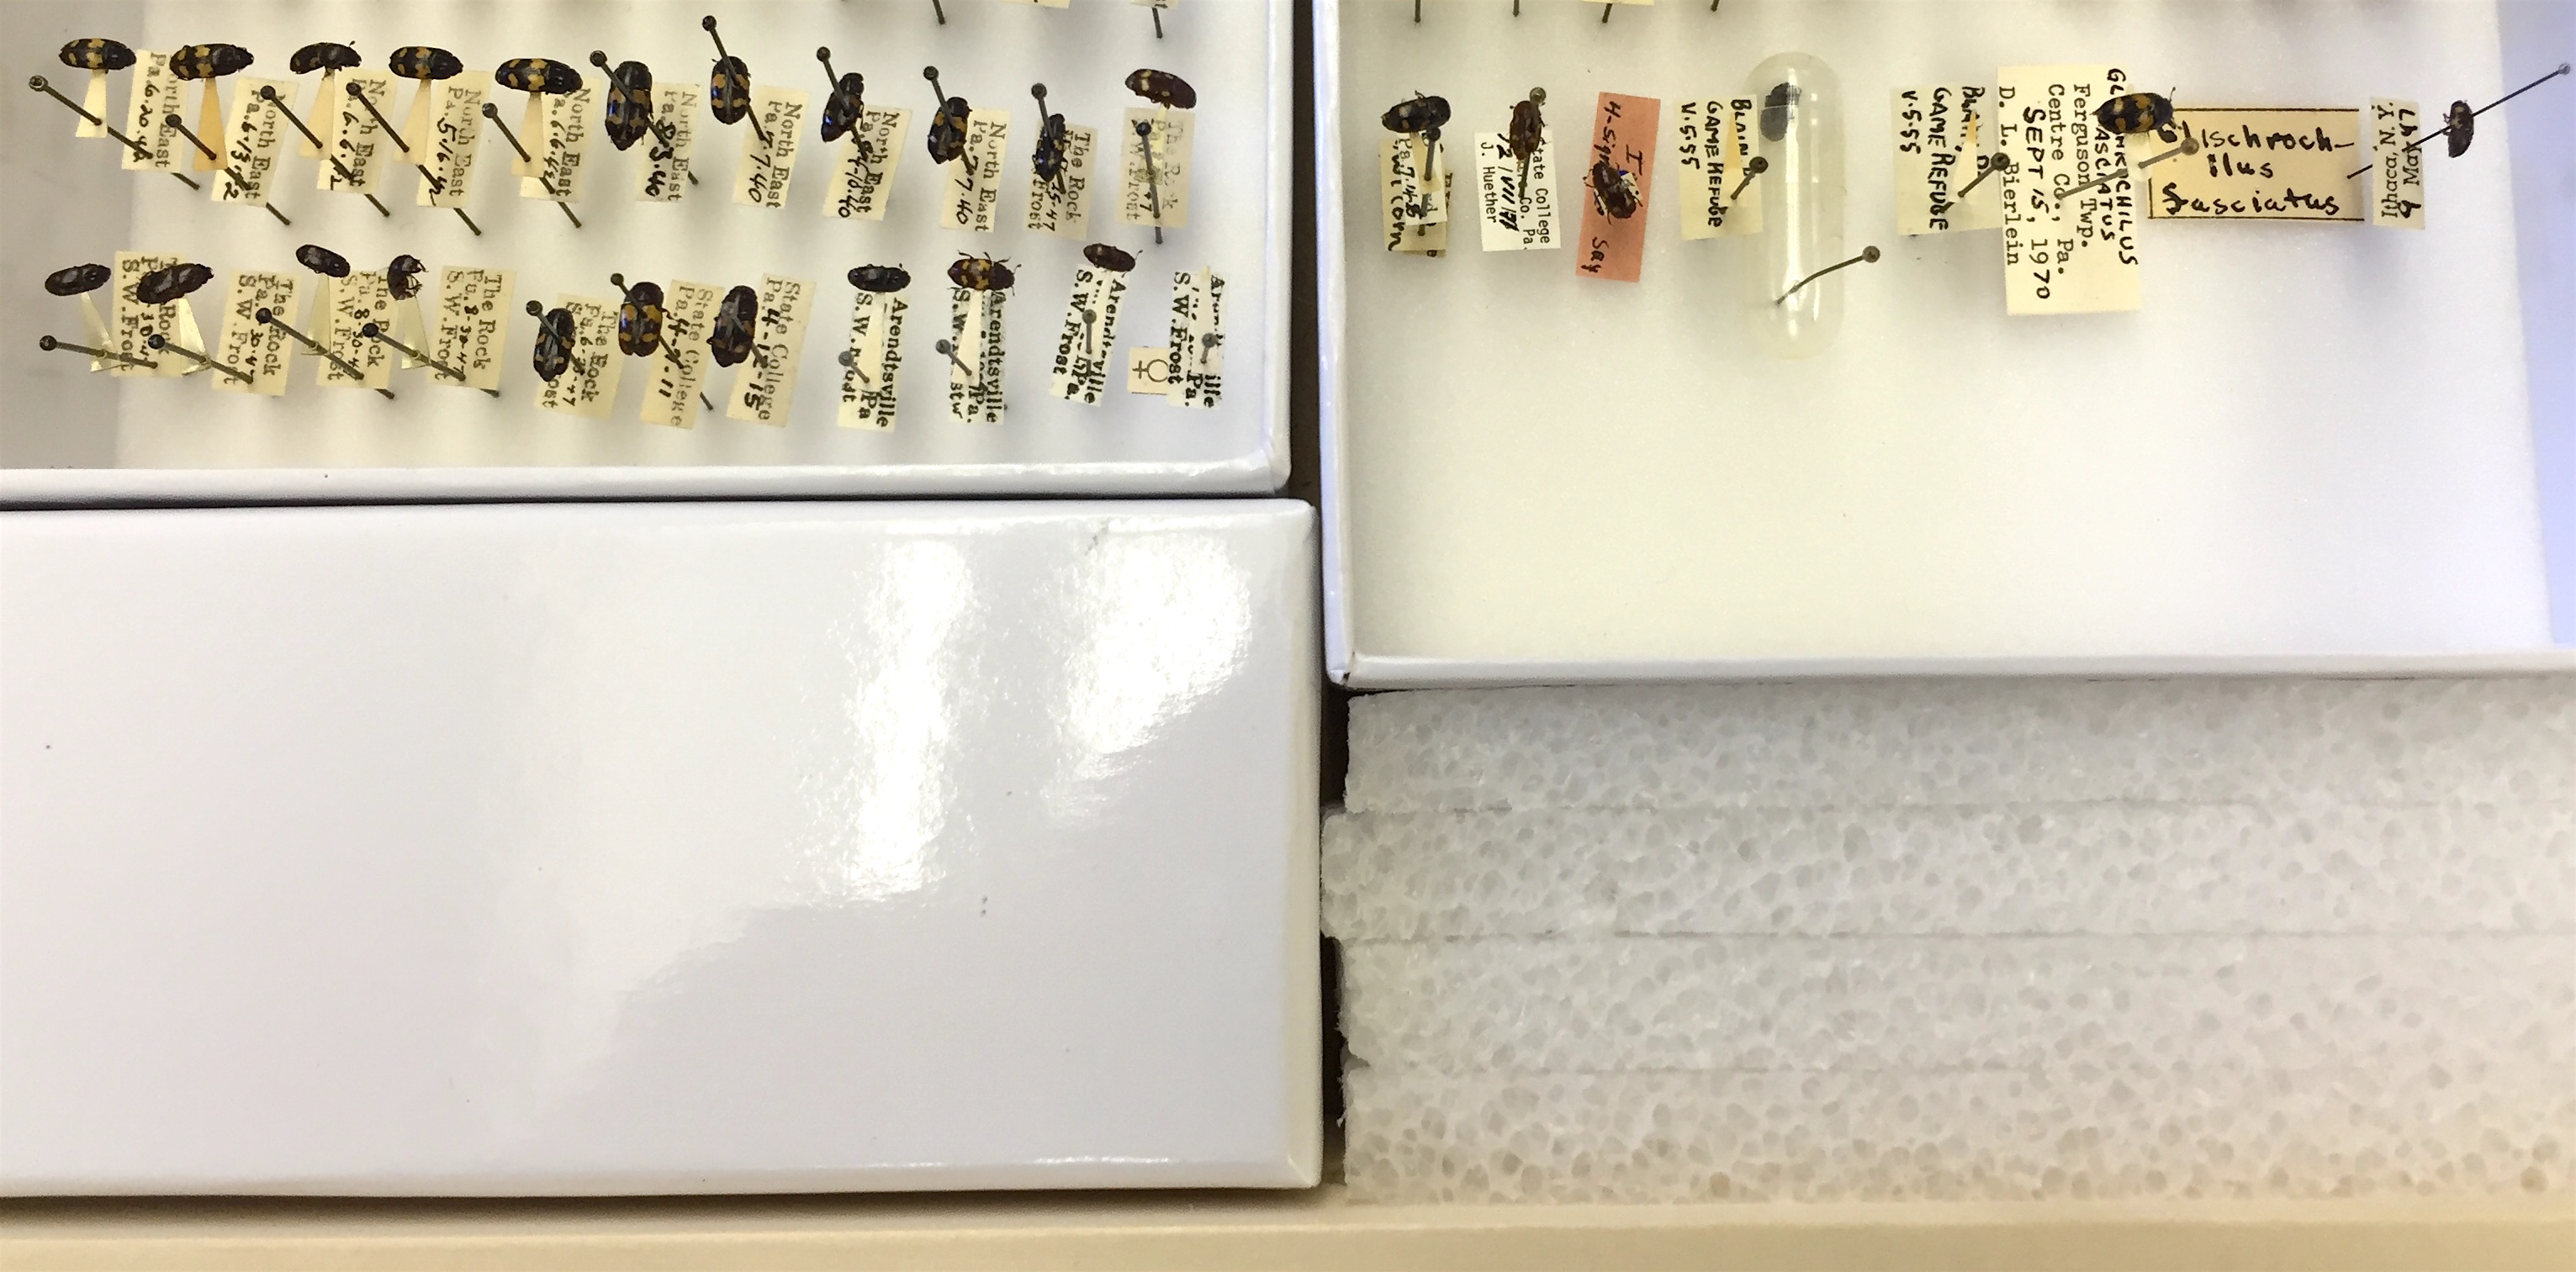
\includegraphics[width=0.75\textwidth]{packedUnitTrays}
  \caption{Empty space filled with unit tray (left) or foam spacers (right). The trays in this drawer are secure. Photo (CC BY 2.0) by Andy Deans.}
  \label{trayspacked}
\end{figure}

\noindent{}Note that each new drawer is marked with a unique number, stamped on both the lid and the drawer (Figure \ref{drawerstamp}). The drawer lid must never be disassociated from its drawer bottom, as they often will not fit other bottoms. One strategy is to place a lid under its drawer bottom after its been removed.\\

\noindent{}For information regarding evidence and treatment of pests see \textit{SOP 02: Museum Pest Management}.\\

\begin{figure}[ht!]
	\centering
  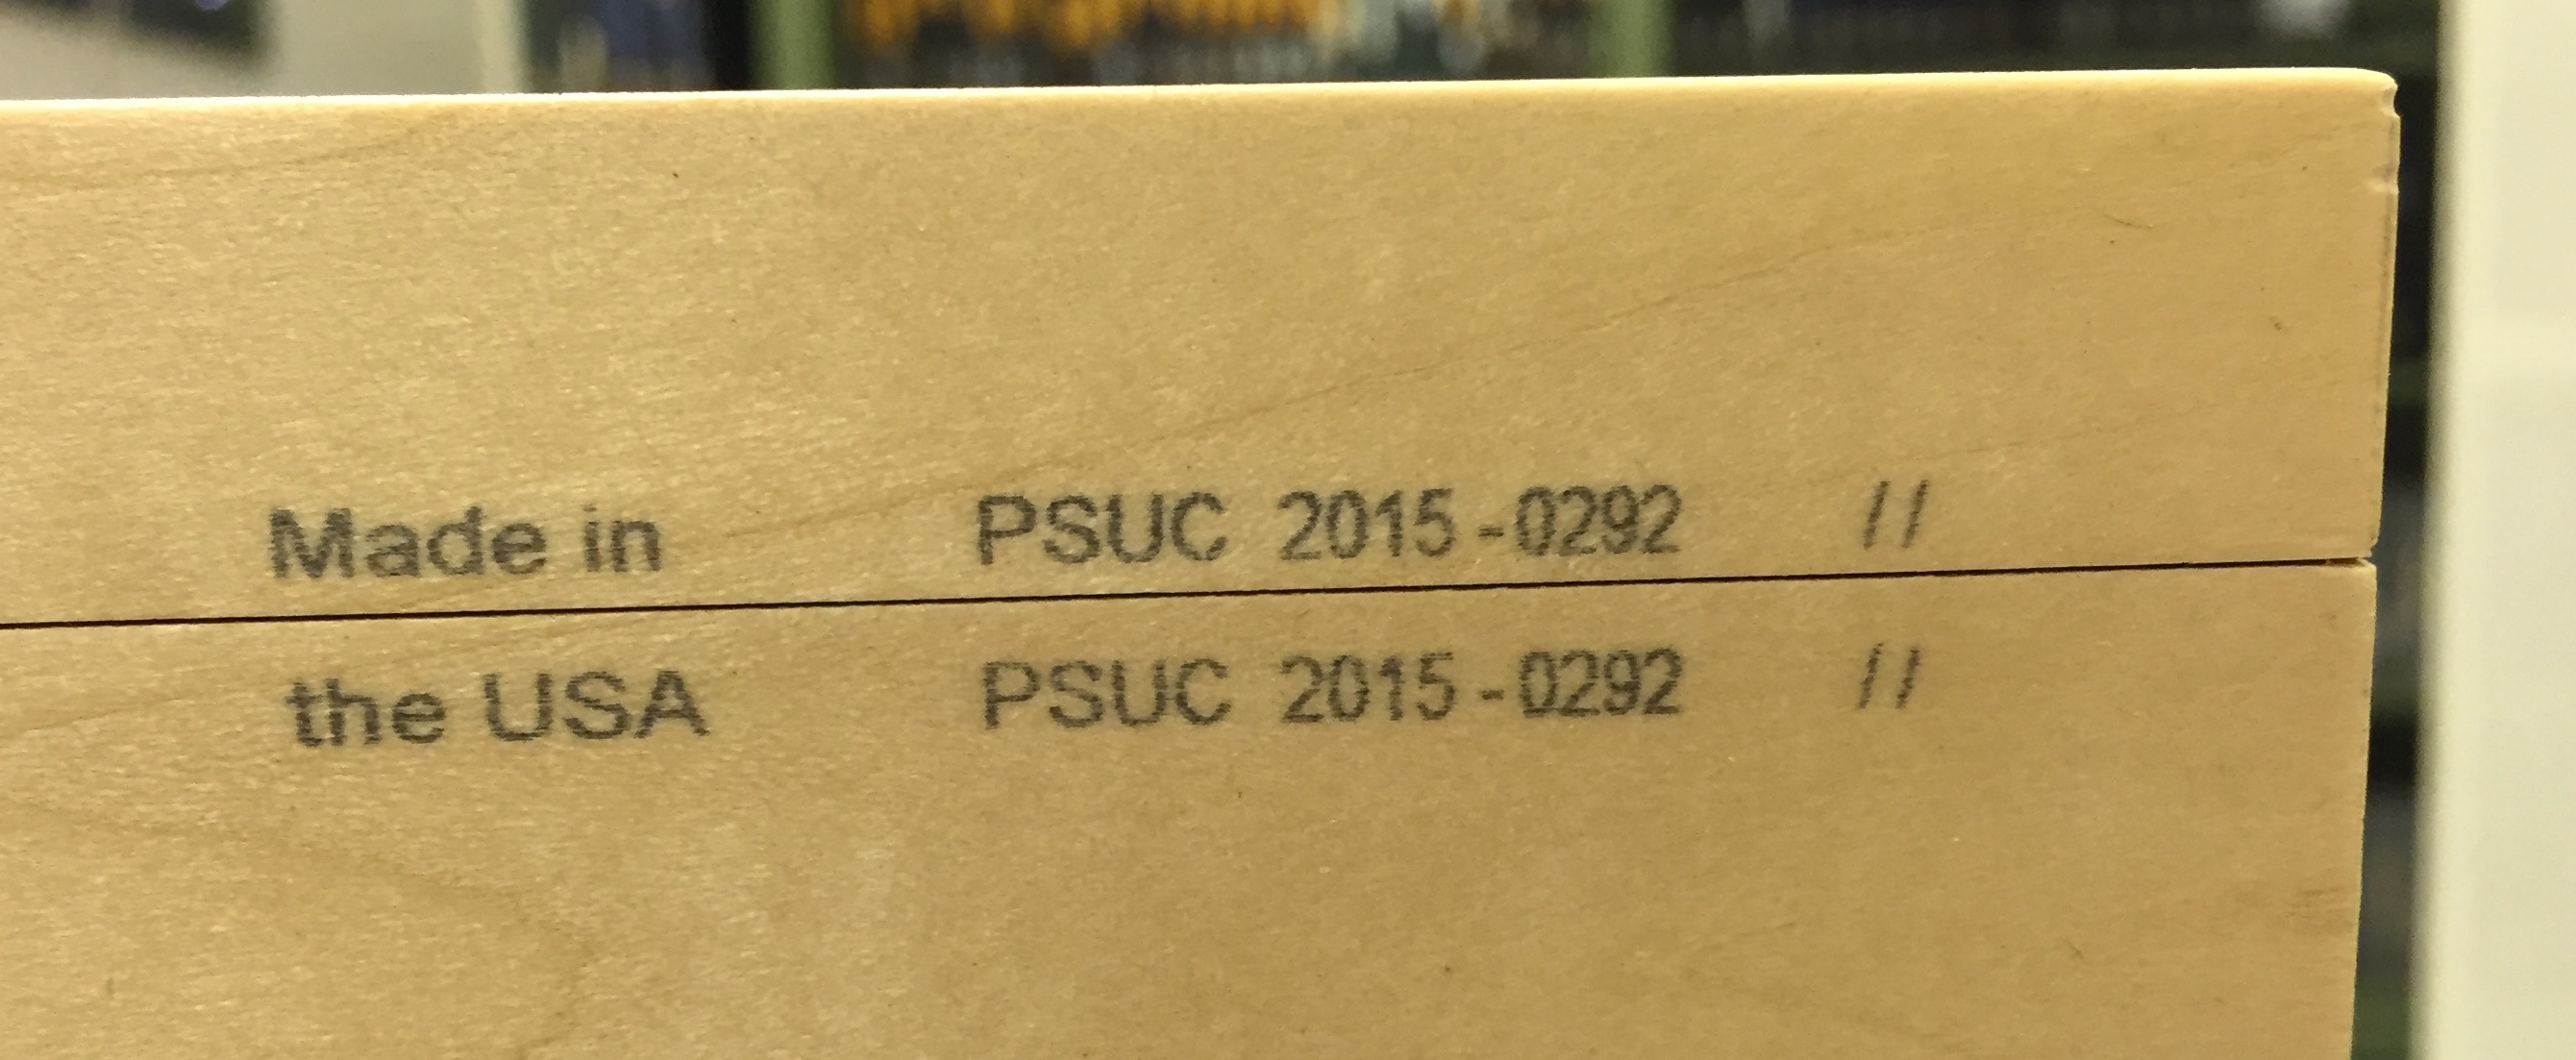
\includegraphics[width=0.75\textwidth]{drawerStamp}
  \caption{Drawer lid and bottom, stamped on the back with their unique number. These numbers better be the same! Photo (CC BY 2.0) by Andy Deans.}
  \label{drawerstamp}
\end{figure}

\subsection{Wet specimen storage equipment}%check vial size
Soft-bodied, aquatic, and other specimens that cannot be stored dry are preserved in $\sim$/80\% ethyl alcohol (ethanol) or 100\% glycerol (glycerine). Frequently accessed specimens are stored in 4 or 8 dram borosilicate glass vials, with black polyseal screw-top lids, and these vials are arranged in cardboard trays. Infrequently accessed specimens are stored in shell vials stopped with polyethylene caps or cotton plugs. These shell vials are arranged inside borosilicate glass jars, topped with ethanol, and fitted with plastic lids that have low-density polyethylene gaskets.

\subsection{Slide specimen storage equipment}
Many slide-mounted specimens are arranged on trays inside a slide cabinet designed by Delta Designs, Ltd. Others are stored inside non-standard array of slide boxes and are likely to be moved to standard 100-slide plastic boxes. Slides must always be stored horizontally.

\subsection{Vendors for storage equipment and supplies}
Cabinets:
\begin{itemize}
\item Delta Designs Ltd., phone: +1 800 656 7426 (ext.219, Brett Danielson), FAX: 785-233-1021, Web: \url{http://www.deltadesignsltd.com}
\item Viking Metal Cabinet Co. Web: \url{http://www.vikingmetal.com/}
\end{itemize}

\noindent{}Dry storage:
\begin{itemize}
\item HH Elements, Inc., \url{http://hhelementsinc.com}, harris@hhelementsinc.com, +1 434 249 8630 (drawers, unit trays, custom small storage)
\item Padgett Manufacturing, 221 Old River Rd, Bridgewater, VA 22812; Don Keagy, donpadgettmfg@verizon.net (drawers)
\end{itemize}

\noindent{}Wet storage:
\begin{itemize}
\item Bioquip Products, Inc., \url{https://www.bioquip.com/} (vials, caps)
\item Wheaton, \url{http://wheaton.com/} (8 and 16 oz., straight-sided jars; LDPE-lined lids)
\end{itemize}

\section{Collection labels protocol}%%work on this; what about numbering jars, etc.?
Label standards vary, depending on the unit to be labeled:
\begin{itemize}
\item Cabinet---Order and families should be printed on a 5$\times$8 card; see cabinet sign template.
\item Drawer---Order and family printed across the top, genera and species below; see drawer sign template.
\item Unit tray---Header card, inserted between foam and tray wall, with genus and species in italics, followed by author and year in Roman. See header card template.
\end{itemize}


%\clearpage
% adding bibliography here
%\bibliographystyle{unsrt}
%\bibliography{bib}

\end{document}

\begin{figure}[ht!]
	\centering
  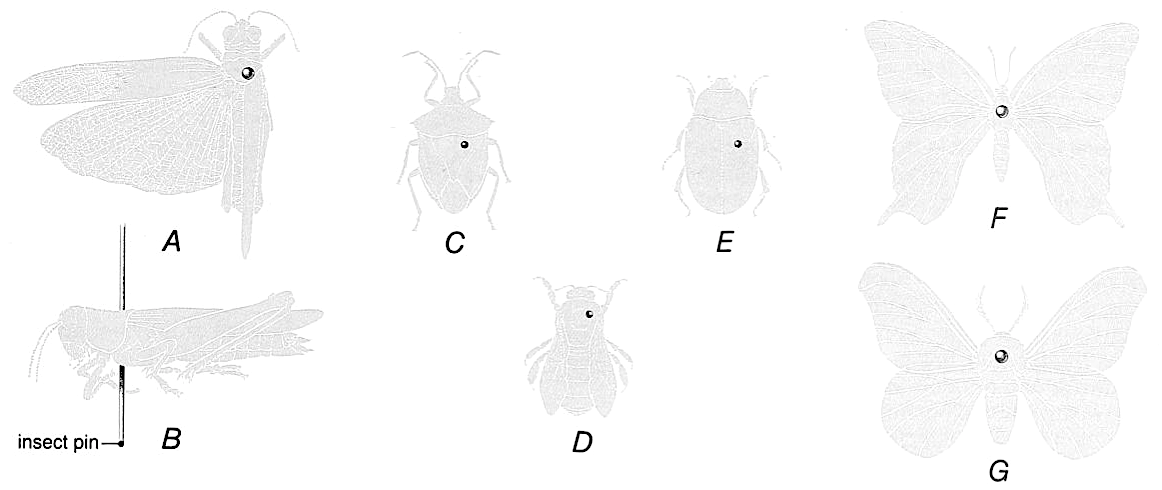
\includegraphics[width=0.75\textwidth]{PinsThorax}
  \caption{Ideal pin placement on different kinds of insects \citep[modified from][Fig. 17]{USDAmanual1986}}
  \label{pinthorax}
\end{figure}

\\

\begin{figure}[ht!]
    \centering
    \begin{subfigure}[ht!]{0.43\textwidth}
        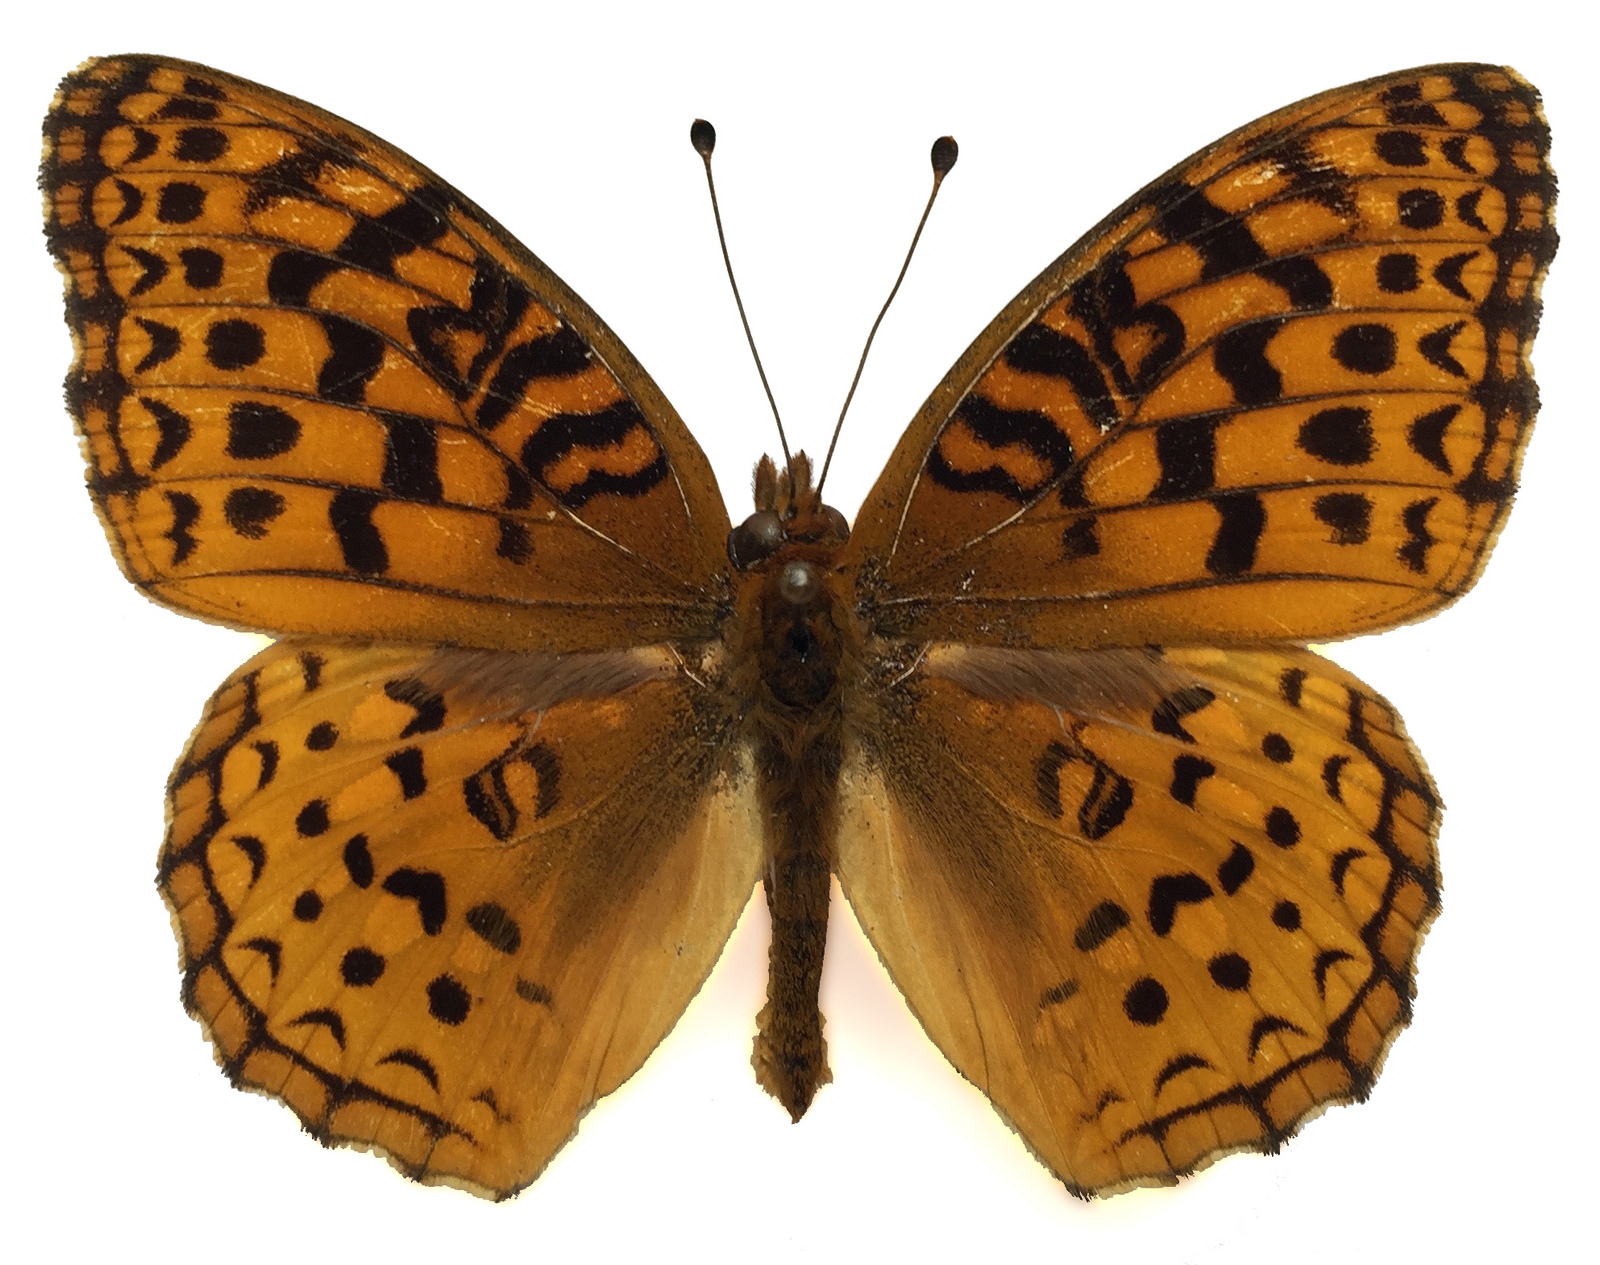
\includegraphics[width=\textwidth]{butterfly}
    \end{subfigure}
    \qquad
    \begin{subfigure}[ht!]{0.45\textwidth}
        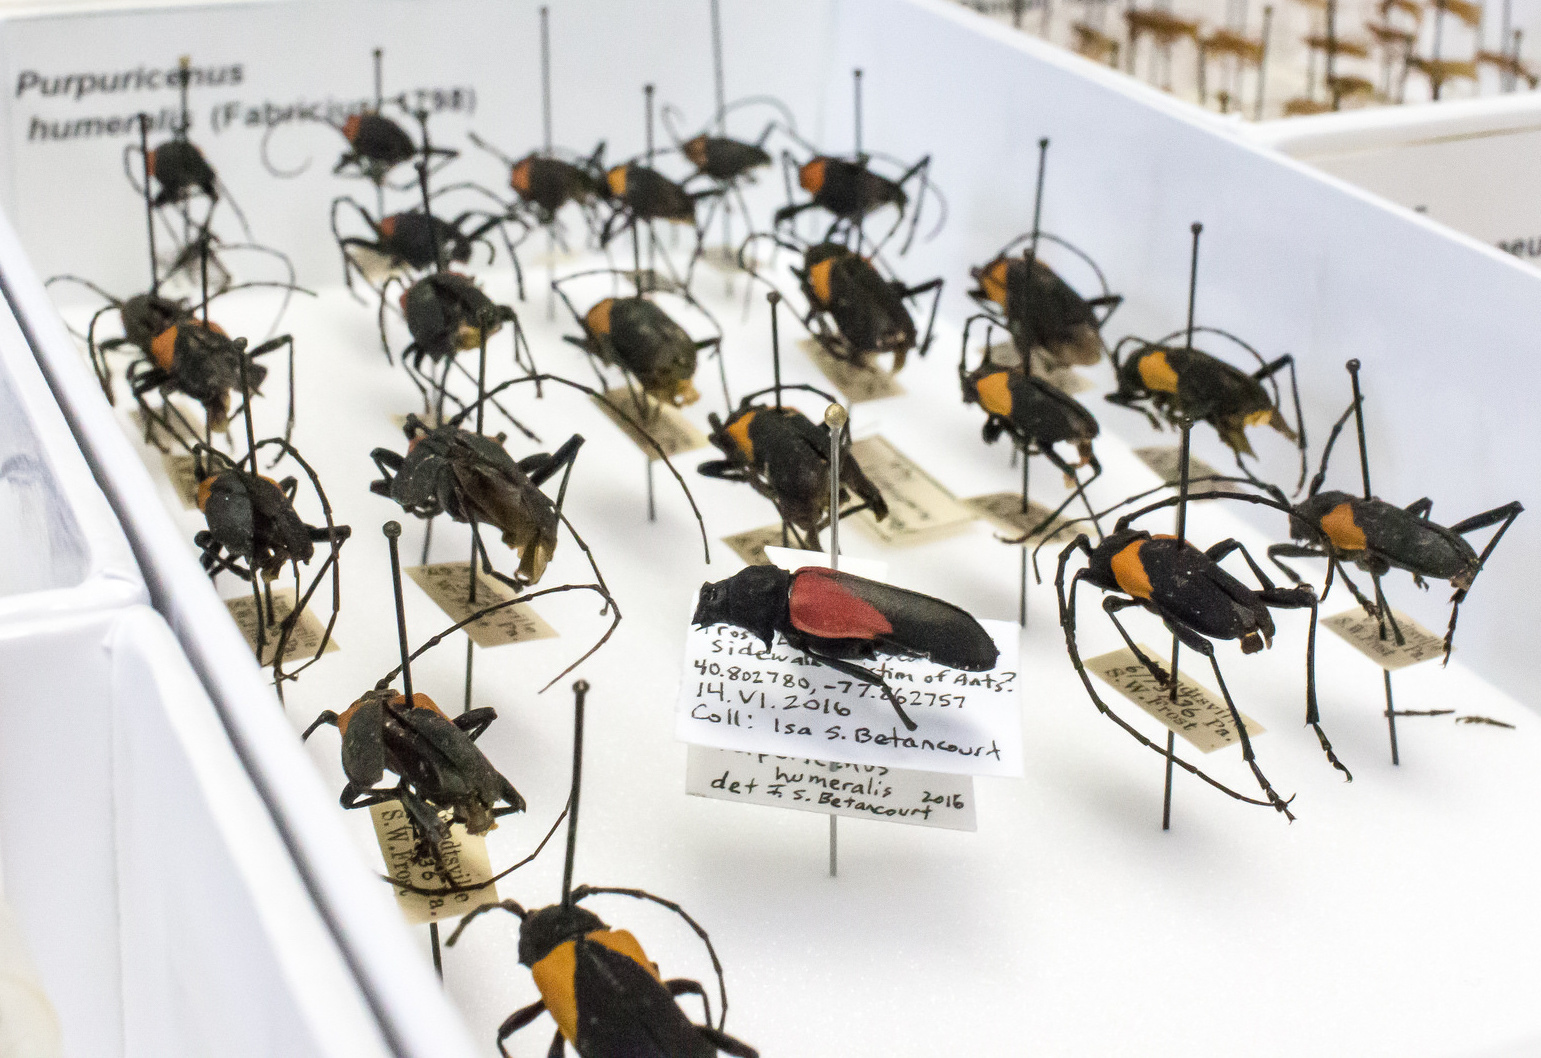
\includegraphics[width=\textwidth]{pinned}
    \end{subfigure}
    \caption{Frost Entomological Museum specimens. Photos CC BY 2.0 by Andy Deans (L) and Isa Betancourt (R)}
\end{figure}